
INSERT FIGURE OF DOFS

It belongs to the Crouzeix-Raviart family. 
The midside nodes are used as degrees of freedom for the velocities.
It is mentioned in Section~6.3 of \textcite{bobf08} (2008): ``[...]
It is exactly divergence free. Another important feature of this
element is that it can be seen as a "mass conservation" scheme. The present element
has been generalized to second order in \textcite{foso83} (1983).
It must also be said that coerciveness may be a problem for the $P_1^{NC} \times P_0$ 
element, as it does not satisfy the discrete version of Korn’s inequality. 
This issue has been deeply investigated and clearly illustrated in \textcite{arno93} (1993).''

At page 170 of \cite{braess} it is stated that ``an analogous quadrilateral element was 
developed and studied by \textcite{ratu92} (1992)''.

\textcite{bobf13}: ``We consider the classical (almost) stable nonconforming triangular 
element introduced in \textcite{crra73}, in which mid-side nodes are used as degrees of 
freedom for the velocities. This generates
a piecewise linear nonconforming approximation; pressures are taken constant on
each element. It is also possible to build a three-dimensional
version of this element, using mid-face nodes as degrees of freedom.''
Also: ``It must also be recalled that coercivity is a problem for the $P_1^{NC}\times P_0$ 
element. The trouble is that the bilinear form (8.2.1) is not coercive on the 
nonconforming space $V_h$ and we do not have the discrete version of Korn's inequality.''

It is also mentioned in \textcite{john16}, appendix B.3, example B.43, in 2D and 3D, 
in \textcite{brfo} (example 8.1), and studied extensively in \textcite{john98} (1998). 

\begin{center}
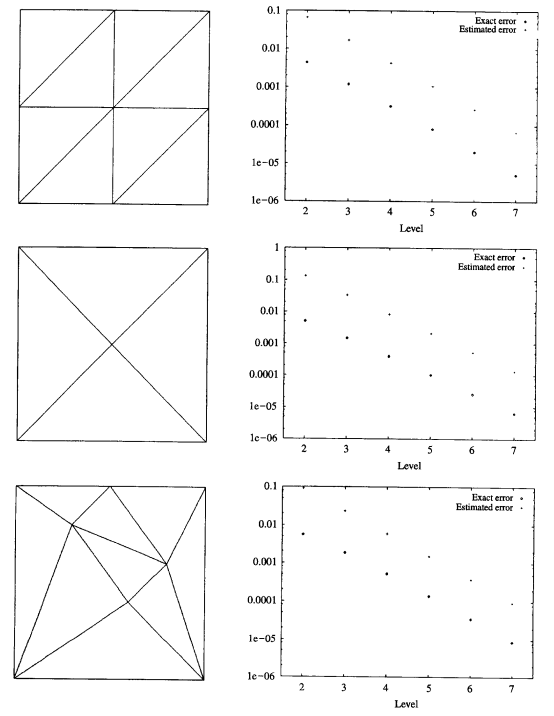
\includegraphics[width=8cm]{images/pair_p1ncp0/john98}\\
{\captionfont Taken from \textcite{john98}.}
\end{center}

